% !TEX TS-program = xelatex
% !TEX encoding = UTF-8 Unicode
% ================================================
%  上海交通大学 研究生工作周报
%  编译: xelatex → bibtex → xelatex → xelatex
% ================================================

\documentclass{sjtuweekly}
\usepackage{booktabs}
\usepackage{tabularx}
\usepackage{array}

% ========== 图表编号: 独立递增 (图1, 表1, ...) ==========
\renewcommand{\thefigure}{\arabic{figure}}
\renewcommand{\thetable}{\arabic{table}}

% ========== 参考文献库 ==========
\bibfile{bib/database}

% ========== 基本信息 ==========
\member{霍锦龙}
\weeknum{xx}

\begin{document}

\makeweeklytitle   % 封面（第1页）

% ================================================
%  正文从第2页开始
% ================================================

\section{一、本周工作概要}

\subsection*{1.1\quad 讨论回顾和周报概要}

基于此前讨论：
\begin{enumerate}
  \item Mixnet文献中对于计算和通信的overlap问题；
  \item vLLM学习；
  \item 故障恢复和OCS损耗建模。
\end{enumerate}

\subsection*{1.2\quad MixNet计算和通信掩盖解决思路}

在前向传播中，提供了两种处理策略：在首次All-to-All通信前，阻塞网络约25ms以等待OCS物理重构完成；第二个是文章提出的MixNet-Copilot 流量预测。利用历史迭代的流量记录和时序加权平均，在上一层的注意力计算阶段提前预测当前层的流量需求。若预测准确则完美隐藏延迟；若存在偏差，则在第二次 All-to-All 时进行微调校准。

\textbf{问题在于} MixNet 在预测失败或首次 All-to-All 时，会将 OCS 重构视为阻塞屏障，导致网络闲置。且依赖历史 Epoch 或上一层的数据进行流量预测本质上是一种“猜测”，在训练初期或数据分布漂移时准确率受限，并且无法为推理阶段重构提供合理支持。最后，MixNet 仅作用于物理/拓扑层，而类似 DeepEP 的优化作用于 CUDA/算子层，两者目前处于割裂状态。\textbf{这些点,可以作为后续研究的内容.}

\subsection*{1.3\quad vLLM学习}

考虑到vllm处在的研究位置表\ref{tab:vllm_moe_ocs_positioning}所示，他可以作为调度或者预测结果的推理验证手段。而在此之前，我们需要通过单机 MoE 进行路由决策分析，先针对单击上MoE路由的数据交换和通信情况做统计图构建和建模。\textbf{如果验证了一些实验假设，并可以利用vllm在推理阶段验证,进行适配性的调整推理需求。}

\begin{table}[htbp]
\centering
\small
\begin{tabularx}{\linewidth}{@{}p{2.4cm}p{3.0cm}X@{}}
\toprule
层级 & 组件 & 在 MoE + OCS 研究中的定位 \\
\midrule

推理/服务层 &
vLLM/SGLang &
作为主要的推理工作负载生成器与观测对象，用于提取 prefill/decode、batching、请求到达、rank 间通信与 collective 行为，并将这些模式作为 OCS 的输入。 \\

研究/原型 API 层 &
Transformers &
作为最灵活的研究接口，适合做最小可复现实验、算法验证和通信 trace 的基础采样。 \\

通信基础设施层 &
OCS &
接收上层抽象出来的通信模式，将其映射到可重构拓扑、链路分配、备份路径或故障恢复策略。 \\

\bottomrule
\end{tabularx}
\caption{vLLM、SGLang、其他 API 与 OCS 在 MoE 场景中的分层定位。}
\label{tab:vllm_moe_ocs_positioning}

\end{table}

在此基础上进行了基于huggingface Transformer网络的模型搭建，\textbf{对 MoE 路由分析工具进行了重构}。包括：

\begin{itemize}
  \item 路由分析子命令验证：\texttt{analyze}负载均衡、熵、专家专业化程度、共激活模式、\texttt{compare}、\texttt{intervene}强制路由、\texttt{ablate}专家消融均已通过基础功能测试
  \item MLX 后端在 Qwen1.5-MoE-A2.7B-Chat-4bit 上完成推理运行，生成 705KB 路由 trace 日志，专家负载分布统计正常
  \item \texttt{schema.py}：统一规范化数据结构 RoutingTrace / TokenRoute / LayerRoute，按绝对 token 位置索引，支持跨层、跨 token 分析
\end{itemize}

\begin{figure}[htbp]
  \centering
  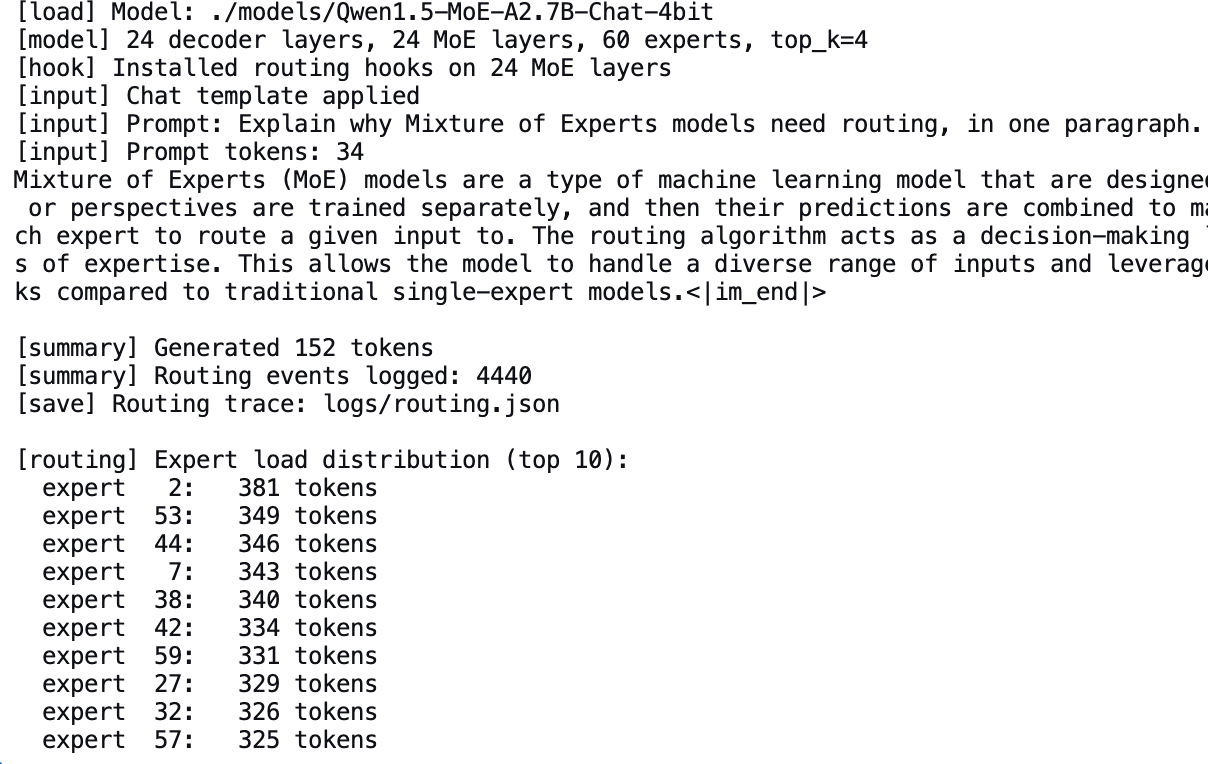
\includegraphics[width=0.85\textwidth]{figures/token分布.png}
  \caption{MoE 路由 Token 在各专家间的分布情况。}
  \label{fig:token_distribution}
\end{figure}

这只是一个初步的结果,其这是基于qwen1.5的混合专家网络模型,\textbf{在不同的推理需求下的路由验证还应该进行大规模验证,并进行建模.}

在验证了不同的路由分布的情况下，在vllm上的研究思路的定位可以为：先用 vLLM 或 SGLang 产生真实的推理/服务负载。记录每个 step 的 phase、batch、rank 对、消息大小和 collective 类型。将 trace 聚类为若干通信模式，例如“大 batch prefill”“小 batch decode”“MoE all-to-all 密集期”“恢复期”等。学习从 workload 特征到通信模式的映射。通信模式进一步映射到 OCS 配置，例如拓扑切换、路径重路由、备份端口选择与恢复策略。在验证了路由的规律和分布情况下，推理侧的vllm也进行了部署后.

最后一步是需要和ocs结合，当前的可提供的验证平台不是很多，主要为：

\begin{itemize}
  \item \textbf{OpenOptics / Optics-Mininet}：提供光数据中心网络的通用开源仿真框架，支持拓扑定义、路由、流量感知调度及控制平面更新逻辑。
  \item \textbf{Etalon}：面向可重构数据中心网络的端到端网络仿真器，侧重于在测试床环境下的可重复实验与复现。
  \item \textbf{Topology Programming Simulator}：用于评估动态光网络重配置对网络弹性与性能影响的纯仿真工具。
  \item \textbf{ns-3 / OMNeT++}：通用离散事件网络仿真底座，无原生 OCS 支持，需开发者自行构建和添加 OCS 行为模型。
\end{itemize}

\textbf{这几个平台，还在逐步了解中。}

\subsection*{1.4\quad 故障恢复和损耗建模}

\textbf{以实际项目/代码的角度出发，几个相关的项目，还未开始学习。}

\textbf{1. OCS 重构、训练恢复与 Checkpoint 优化}

\begin{itemize}
  \item {ReNoVatE}：将节点故障后的 rank 备份、检查点选取和路径重映射，抽象为虚拟网络局部重嵌入的数学恢复优化问题。
  \item {DLRover}：提供容错、自动扩缩容和 Flash Checkpoint，实现基于内存检查点的秒级失败训练恢复。
  \item {NVIDIA cuda-checkpoint + CRIU}：结合 CUDA 运行状态与 CRIU 技术，实现系统底层的透明检查点与恢复。
  \item {Oobleck}：利用流水线模板和故障后的动态重配置来实现分布式训练容错。
  \item {Bamboo}：面向抢占式实例，利用流水线气泡实现低暂停的训练恢复。
  \item {GEMINI}：利用内存检查点进行分布式训练，侧重于研究检查点服务器的选址、网络距离与恢复代价的优化。
\end{itemize}

\textbf{2. 新型硬件损耗建模、实现与资源优化}

\begin{itemize}
  \item {OpenOptics}：解耦光数据中心网络软硬件的开放框架，通过 time-flow table 统一接口，支持自定义光网络的仿真与部署。
  \item {GNPy}：面向真实网状光网络的开源路由规划库，用于开发生产级的路径规划与网络资源优化工具。
  \item {HARF-drawing}：用于计算管状反谐振空心光纤制造和拉丝参数的开源物理仿真工具。
  \item {FiberModeSolver}：基于有限差分法求解波动方程，用于光纤传播模态、光场限制和损耗的基础物理建模。
  \item {OIDT (Optical Interconnect Designer Tool)}：提供 FDTD、S 参数提取等功能，用于光互联器件级别的物理与等效电路建模。
  \item {GDSFactory}：支持光子芯片设计、仿真和优化的开源代码库，用于构建损耗感知的芯片设计流程。
  \item {HC-ARF}：利用监督学习直接预测空心反谐振光纤的传播损耗，作为“损耗建模+资源优化”研究的机器学习基线。
\end{itemize}

% ================================================
\section{二、遇到的问题与讨论}

\begin{enumerate}
  \item \textbf{token在训练侧的分布情况不清晰}：\texttt{moe\_run.py} 当前的问题主要集中在，是使用已有的模型权重进行推理侧的验证，即使是token在不同专家中的分布，仍然是推理侧，应该转向，训练端，从数据的角度出发，首先在训练侧了解数据的偏好分布，之后利用有效预测，在推理端验证。
  \item \textbf{Qwen3.5-MoE 模型结构差异}：Qwen3.5-MoE 的 decoder layers 嵌套在 \texttt{language\_model} 子模块中（区别于 Qwen1.5-MoE 的扁平结构），在 \texttt{model\_utils.py} 中通过 \texttt{\_find\_decoder\_layers()} 适配，但后续新增 MoE 架构变体时仍需维护适配逻辑。
\end{enumerate}

% ================================================
\section{三、工作计划}

\begin{enumerate}
  \item 完成训练侧即使是合成数据的模型训练侧的路由和通信图构建，讨论数据的分布情况。基于 LoRA 微调后的 adapter 进行路由对比实验，评估微调对 expert routing 行为的影响.
  \item 并在 Qwen3.6-35B-A3B-4bit 上运行完整路由分析流程，产出专家负载分布与专业化程度的量化结果.
  \item 尝试利用先验知识结合vllm进行推理指导.
  \item 学习ocs相关仿真.
\end{enumerate}

% ================================================
\printbib

\end{document}
